\documentclass[11pt,compress,t,notes=noshow, xcolor=table]{beamer}
\usepackage[]{graphicx}\usepackage[]{color}
% maxwidth is the original width if it is less than linewidth
% otherwise use linewidth (to make sure the graphics do not exceed the margin)
\makeatletter
\def\maxwidth{ %
  \ifdim\Gin@nat@width>\linewidth
    \linewidth
  \else
    \Gin@nat@width
  \fi
}
\makeatother

\newcommand{\citebutton}[2]{%
\beamergotobutton{\href{#2}{#1}}%
}

\newcommand{\blu}[1]{\textcolor{blue}{#1}}
\newcommand{\org}[1]{\textcolor{orange}{#1}}
\newcommand{\ques}{\textbf{\textcolor{red}{Question:  }}}
\newcommand{\questionssofar}{\begin{frame}\frametitle{Any questions?}\end{frame}}

\newcommand\warning{%
 \makebox[1.4em][c]{%
 \makebox[0pt][c]{\raisebox{.1em}{\scriptsize!}}%
 \makebox[0pt][c]{\color{red}\normalsize$\bigtriangleup$}}}%

\definecolor{fgcolor}{rgb}{0.345, 0.345, 0.345}
\newcommand{\hlnum}[1]{\textcolor[rgb]{0.686,0.059,0.569}{#1}}%
\newcommand{\hlstr}[1]{\textcolor[rgb]{0.192,0.494,0.8}{#1}}%
\newcommand{\hlcom}[1]{\textcolor[rgb]{0.678,0.584,0.686}{\textit{#1}}}%
\newcommand{\hlopt}[1]{\textcolor[rgb]{0,0,0}{#1}}%
\newcommand{\hlstd}[1]{\textcolor[rgb]{0.345,0.345,0.345}{#1}}%
\newcommand{\hlkwa}[1]{\textcolor[rgb]{0.161,0.373,0.58}{\textbf{#1}}}%
\newcommand{\hlkwb}[1]{\textcolor[rgb]{0.69,0.353,0.396}{#1}}%
\newcommand{\hlkwc}[1]{\textcolor[rgb]{0.333,0.667,0.333}{#1}}%
\newcommand{\hlkwd}[1]{\textcolor[rgb]{0.737,0.353,0.396}{\textbf{#1}}}%
\let\hlipl\hlkwb

\usepackage{framed}
\makeatletter
\newenvironment{kframe}{%
 \def\at@end@of@kframe{}%
 \ifinner\ifhmode%
  \def\at@end@of@kframe{\end{minipage}}%
  \begin{minipage}{\columnwidth}%
 \fi\fi%
 \def\FrameCommand##1{\hskip\@totalleftmargin \hskip-\fboxsep
 \colorbox{shadecolor}{##1}\hskip-\fboxsep
     % There is no \\@totalrightmargin, so:
     \hskip-\linewidth \hskip-\@totalleftmargin \hskip\columnwidth}%
 \MakeFramed {\advance\hsize-\width
   \@totalleftmargin\z@ \linewidth\hsize
   \@setminipage}}%
 {\par\unskip\endMakeFramed%
 \at@end@of@kframe}
\makeatother

\definecolor{shadecolor}{rgb}{.97, .97, .97}
\definecolor{messagecolor}{rgb}{0, 0, 0}
\definecolor{warningcolor}{rgb}{1, 0, 1}
\definecolor{errorcolor}{rgb}{1, 0, 0}
\newenvironment{knitrout}{}{} % an empty environment to be redefined in TeX

\usepackage{alltt}
\newcommand{\SweaveOpts}[1]{}  % do not interfere with LaTeX
\newcommand{\SweaveInput}[1]{} % because they are not real TeX commands
\newcommand{\Sexpr}[1]{}       % will only be parsed by R
\newcommand{\xmark}{\ding{55}}%


\usepackage[english]{babel}
\usepackage[utf8]{inputenc}

\usepackage{dsfont}
\usepackage{verbatim}
\usepackage{amsmath}
\usepackage{amsfonts}
\usepackage{amssymb}
\usepackage{bm}
\usepackage{csquotes}
\usepackage{multirow}
\usepackage{longtable}
\usepackage{booktabs}
\usepackage{enumerate}
\usepackage[absolute,overlay]{textpos}
\usepackage{psfrag}
\usepackage{algorithm}
\usepackage{algpseudocode}
\usepackage{eqnarray}
\usepackage{arydshln}
\usepackage{tabularx}
\usepackage{placeins}
\usepackage{tikz}
\usepackage{setspace}
\usepackage{colortbl}
\usepackage{mathtools}
\usepackage{wrapfig}
\usepackage{bm}
\usepackage{amsmath}
\usepackage{pifont}

\usetikzlibrary{shapes.multipart,shapes,arrows,automata,positioning,calc,chains,trees, shadows}
\tikzset{
  %Define standard arrow tip
  >=stealth',
  %Define style for boxes
  punkt/.style={
    rectangle,
    rounded corners,
    draw=black, very thick,
    text width=6.5em,
    minimum height=2em,
    text centered},
  % Define arrow style
  pil/.style={
    ->,
    thick,
    shorten <=2pt,
    shorten >=2pt,}
}

\tikzstyle{vec}=[draw, rectangle, fill = white, minimum width=5mm, minimum height=1cm, inner sep = 2pt]

\usepackage{subfig}

% Defines macros and environments
\usepackage{../../style/lmu-lecture}


\let\code=\texttt
\let\proglang=\textsf

\setkeys{Gin}{width=0.9\textwidth}

\setbeamertemplate{frametitle}{\expandafter\uppercase\expandafter\insertframetitle}

\usepackage{bbm}
% basic latex stuff
\newcommand{\pkg}[1]{{\fontseries{b}\selectfont #1}} %fontstyle for R packages
\newcommand{\lz}{\vspace{0.5cm}} %vertical space
\newcommand{\dlz}{\vspace{1cm}} %double vertical space
\newcommand{\oneliner}[1] % Oneliner for important statements
{\begin{block}{}\begin{center}\begin{Large}#1\end{Large}\end{center}\end{block}}


%new environments
\newenvironment{vbframe}  %frame with breaks and verbatim
{
 \begin{frame}[containsverbatim,allowframebreaks]
}
{
\end{frame}
}

\newenvironment{vframe}  %frame with verbatim without breaks (to avoid numbering one slided frames)
{
 \begin{frame}[containsverbatim]
}
{
\end{frame}
}

\newenvironment{blocki}[1]   % itemize block
{
 \begin{block}{#1}\begin{itemize}
}
{
\end{itemize}\end{block}
}

\newenvironment{fragileframe}[2]{  %fragile frame with framebreaks
\begin{frame}[allowframebreaks, fragile, environment = fragileframe]
\frametitle{#1}
#2}
{\end{frame}}


\newcommand{\myframe}[2]{  %short for frame with framebreaks
\begin{frame}[allowframebreaks]
\frametitle{#1}
#2
\end{frame}}

\newcommand{\remark}[1]{
  \textbf{Remark:} #1
}


\newenvironment{deleteframe}
{
\begingroup
\usebackgroundtemplate{
\includegraphics[width=\paperwidth,height=\paperheight]{../style/color/red.png}}
 \begin{frame}
}
{
\end{frame}
\endgroup
}
\newenvironment{simplifyframe}
{
\begingroup
\usebackgroundtemplate{
\includegraphics[width=\paperwidth,height=\paperheight]{../style/color/yellow.png}}
 \begin{frame}
}
{
\end{frame}
\endgroup
}\newenvironment{draftframe}
{
\begingroup
\usebackgroundtemplate{
\includegraphics[width=\paperwidth,height=\paperheight]{../style/color/green.jpg}}
 \begin{frame}
}
{
\end{frame}
\endgroup
}
% https://tex.stackexchange.com/a/261480: textcolor that works in mathmode
\makeatletter
\renewcommand*{\@textcolor}[3]{%
  \protect\leavevmode
  \begingroup
    \color#1{#2}#3%
  \endgroup
}
\makeatother





\input{../../latex-math/basic-math.tex}
\input{../../latex-math/basic-ml.tex}

\newcommand{\titlefigure}{figure/ml-basic-riskmin-error-surface.png}
\newcommand{\learninggoals}{\item Know the concept of loss \item Understand the relationship between loss and risk \item Understand the relationship between risk minimization and finding the best model}

\title{Introduction to Machine Learning}
% \author{Bernd Bischl, Christoph Molnar, Daniel Schalk, Fabian Scheipl}
\institute{\href{https://compstat-lmu.github.io/lecture_i2ml/}{compstat-lmu.github.io/lecture\_i2ml}}
\date{}
\begin{document}

\lecturechapter{ML-Basics: Losses \& Risk Minimization}
\lecture{Introduction to Machine Learning}

\begin{vbframe}{How to Evaluate Models}

\begin{itemize}
\item When training a learner, we optimize over our hypothesis space,
    to find the function which matches our training data best.
\item This means, we are looking for a function, where the 
    predicted output per training point is as close as possible to
    the observed label.
\end{itemize}


% % FIGURE SOURCE: https://docs.google.com/presentation/d/1dTc5act2POjELGuD8wFIUbPxG0QRZlg1PaYdHGU-FJM/edit?usp=sharing
% \begin{center}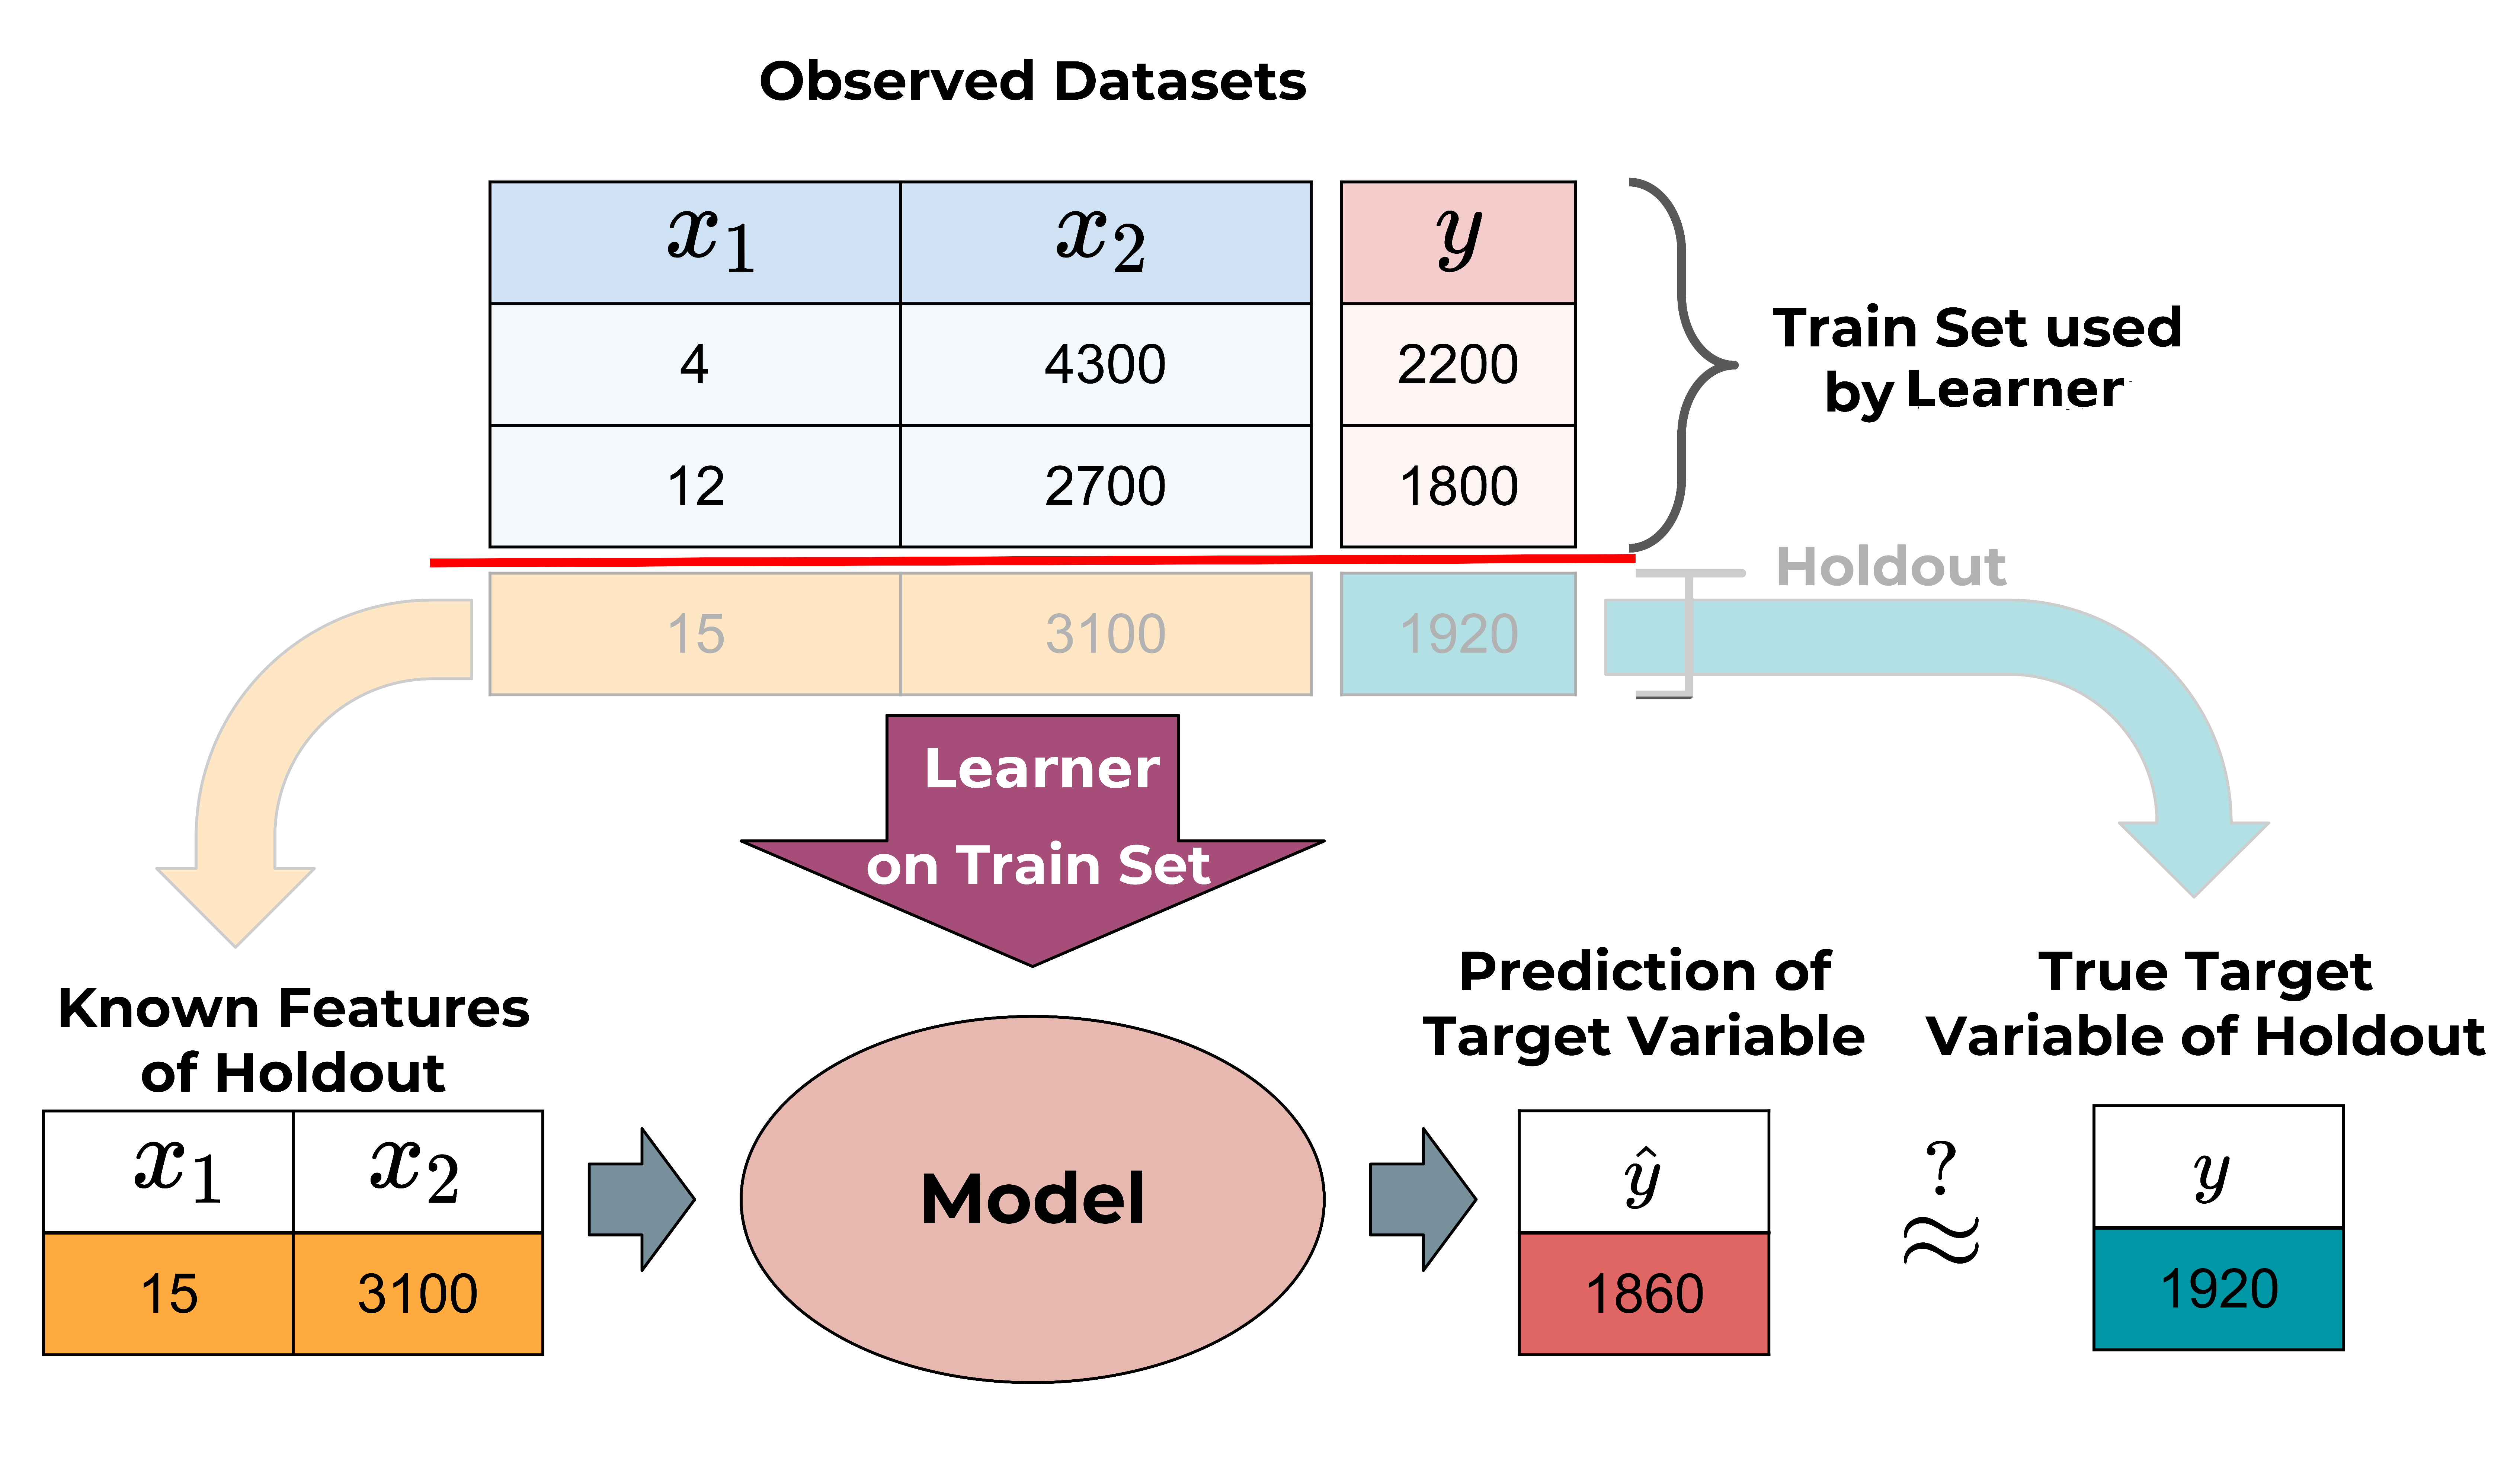
\includegraphics[width=0.8\textwidth]{figure_man/eval_inducer1_web} \end{center}

%https://docs.google.com/presentation/d/1l3VlmPYZs_ycbAIVet05lBcCGEbQeUCl3CAG56BllvM/edit?usp=sharing page 1


\begin{center}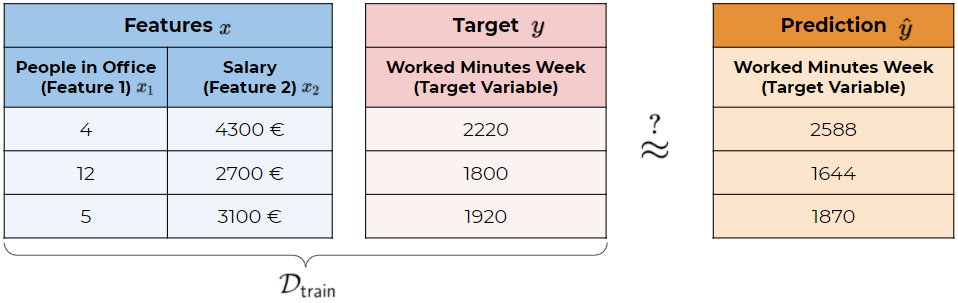
\includegraphics[width=0.8\textwidth]{figure_man/ml-basics-riskmin-eval.png} \end{center}
% \vspace{-0.5cm}
\begin{itemize}
    \item To make this precise, we need to define now how we measure the difference
        between a prediction and a ground truth label pointwise.
%     \begin{itemize}
%       \item Absolute error $|2588 - 2220| = 368$
%       \item Squared error: $(2588 - 2220)^2 = 135,424$\\
%     \end{itemize}
%     \item The choice of this metric has a major influence on the final model, as it determines what a \emph{good} model is. 
%     \item It will determine the ranking of the different models $f \in \Hspace$.
%     \item The metric we use is called the \textbf{loss function}. 
  \end{itemize}
  
\end{vbframe}


\begin{vbframe}{Loss}

The \textbf{loss function} $\Lxy$ quantifies the "quality" of the prediction $\fx$ of a single observation $\xv$:
    $$
    L: \Yspace \times \R^g \to \R.
    $$
In regression, we could use the absolute loss $\Lxy = |\fx - y|$; 


% \vfill


%ml-basic-riskmin-1-loss.R first plot
% \begin{center}
% \begin{figure}[!b]

\begin{center}
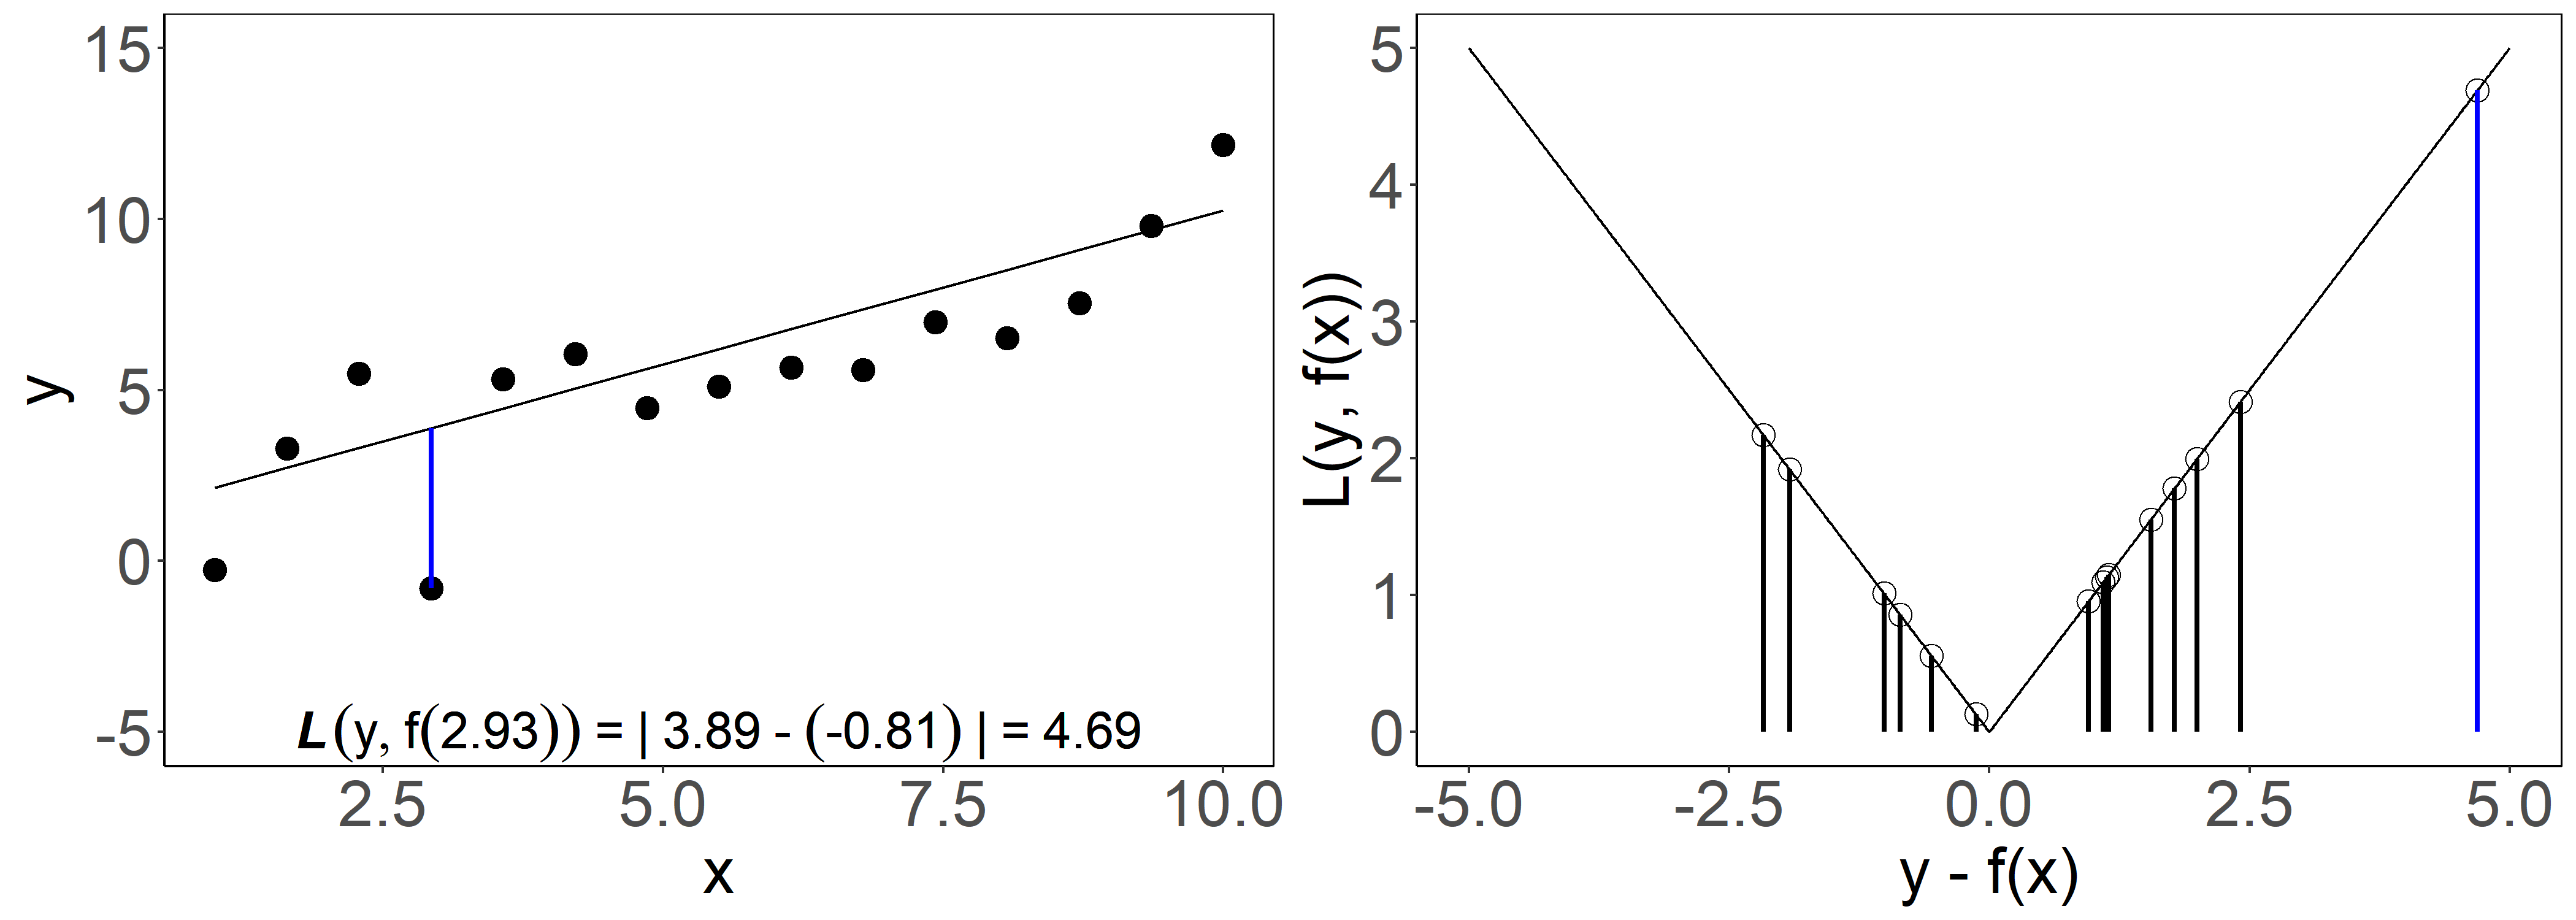
\includegraphics[width=0.5\textwidth]{figure/ml-basic_riskmin-1-loss_abs.png}
\end{center}
or the L2-loss $\Lxy = (y - \fx)^2$:
\begin{center}
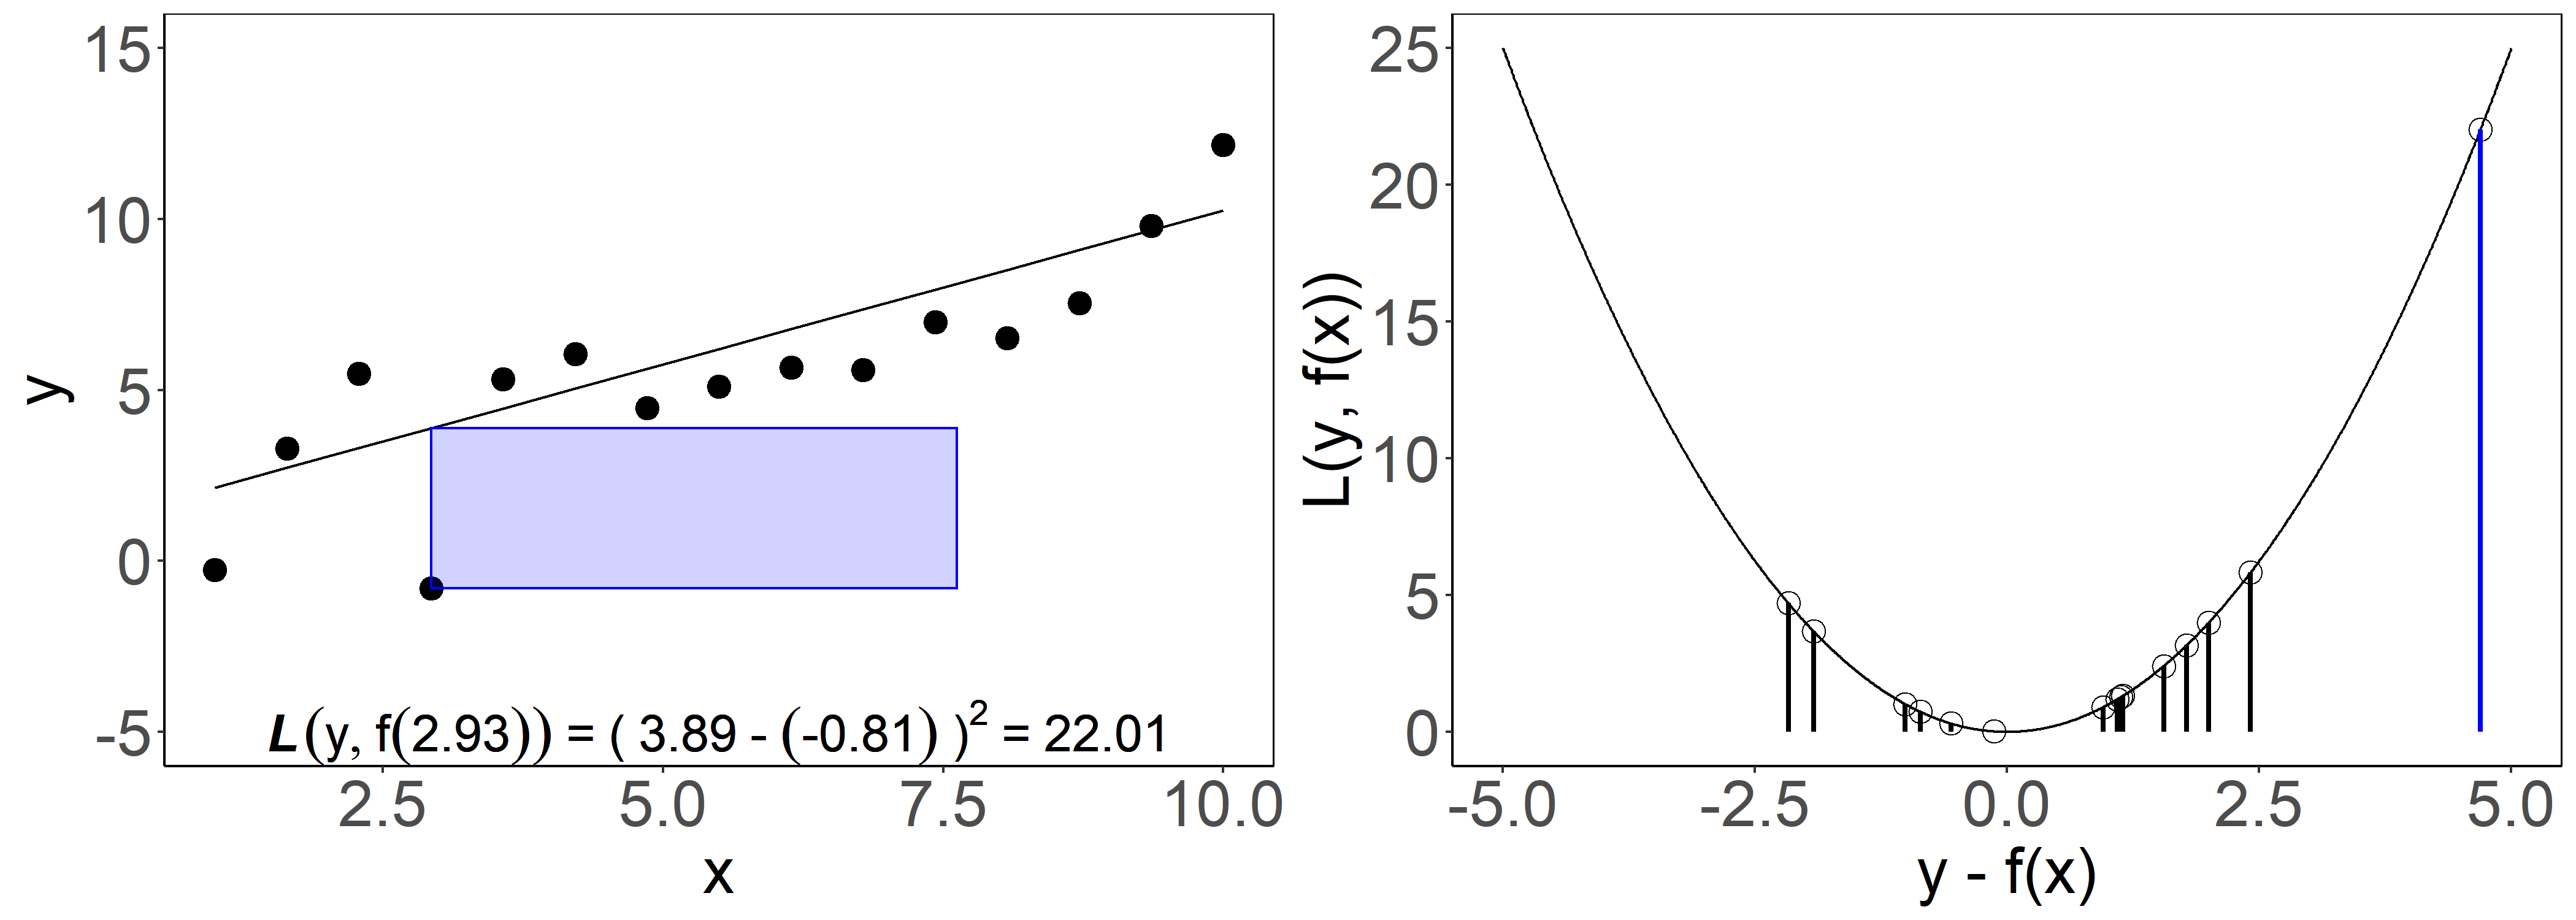
\includegraphics[width=0.5\textwidth]{figure/ml-basic_riskmin-1-loss_sqrd.png}
\end{center}
% \end{figure}
% \end{center}


%ml-basic-riskmin-1-loss.R first plot
% \begin{center}
% \begin{figure}[!b]
% 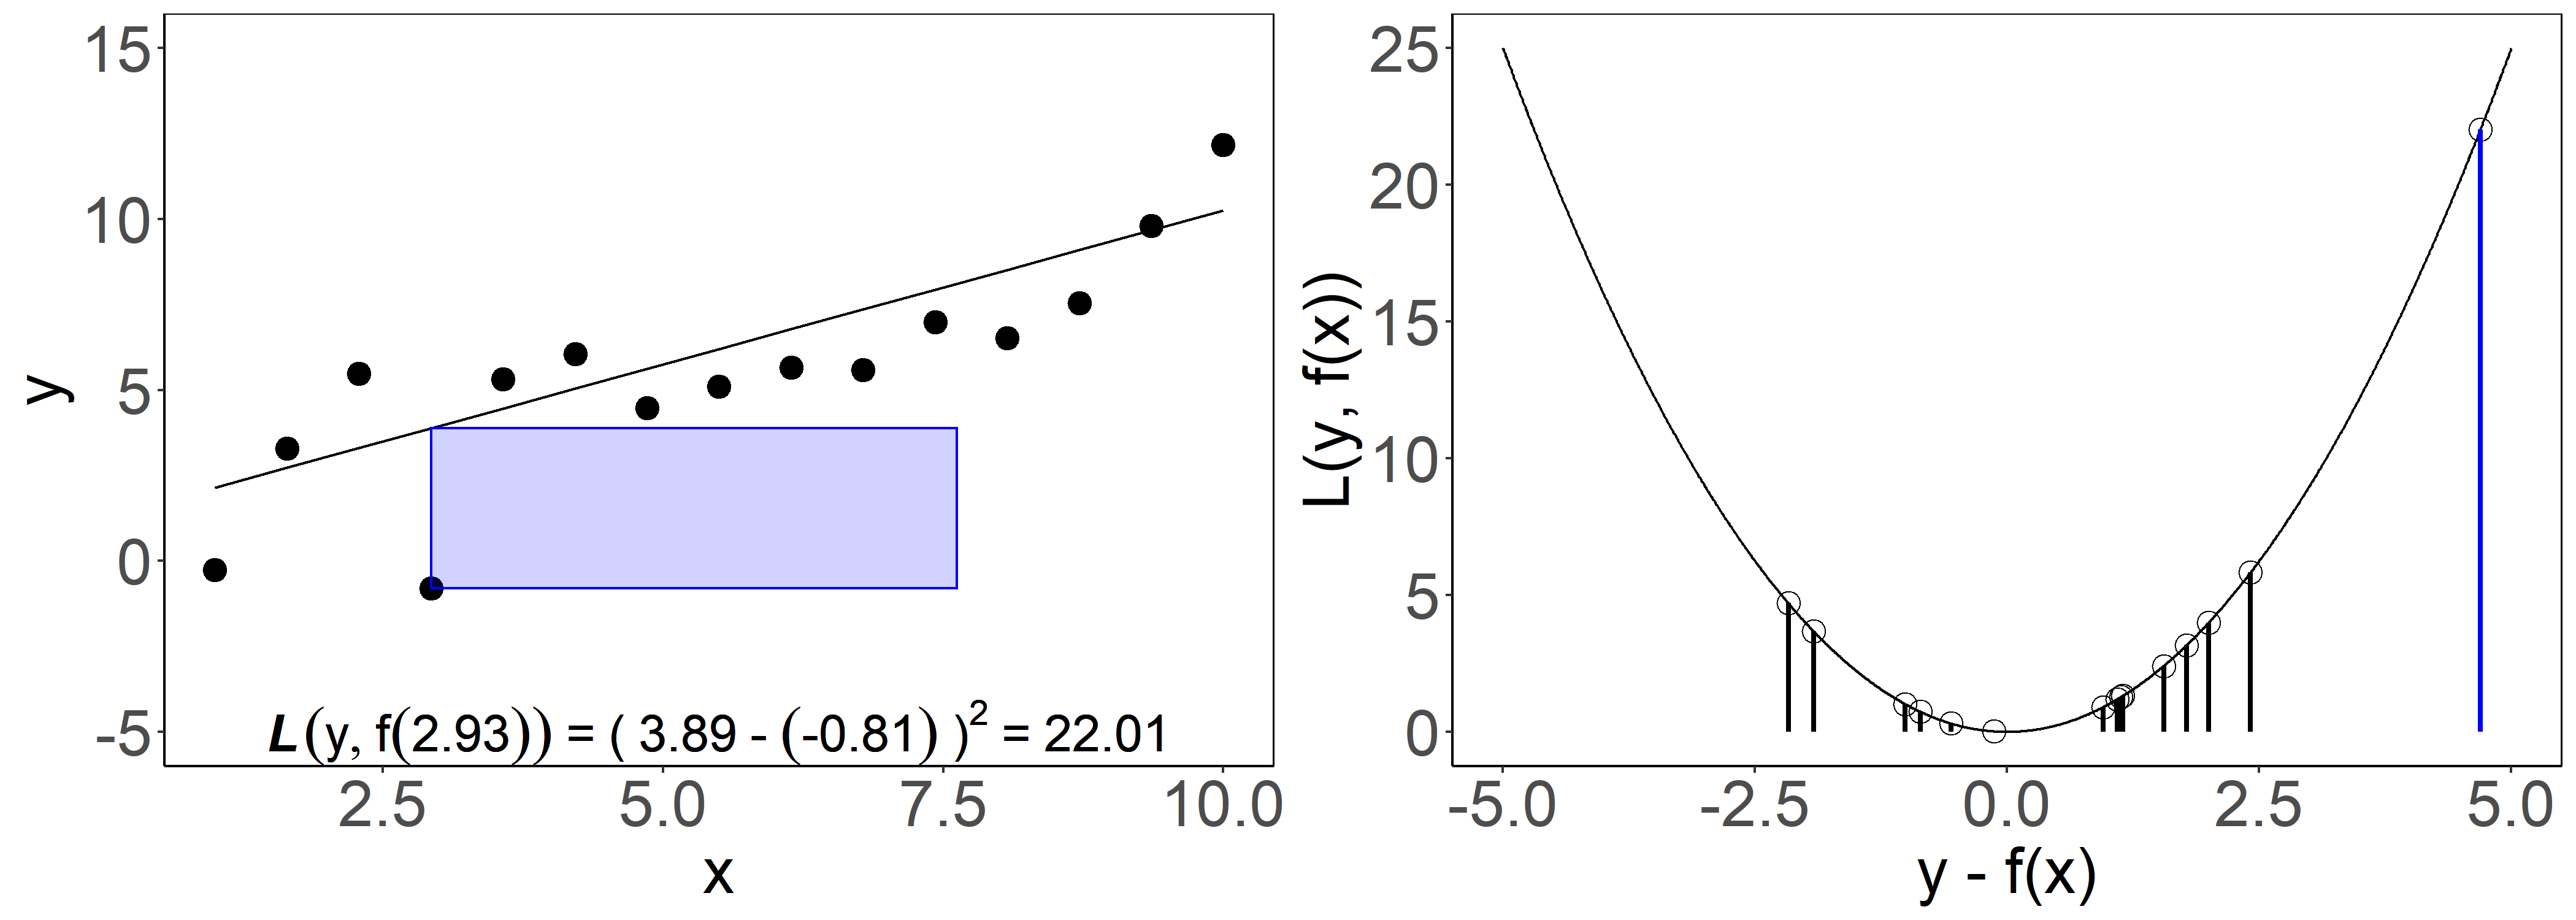
\includegraphics[width=0.5\textwidth]{figure/ml-basic_riskmin-1-loss_sqrd.png}
% \end{figure}
% \end{center}



\end{vbframe}


\begin{vbframe}{Risk of a Model}

\begin{itemize}
  \item The (theoretical) \textbf{risk} associated with a certain hypothesis $\fx$ measured by a loss function $\Lxy$ is the \textbf{expected loss}
  $$ \riskf := \E_{xy} [\Lxy] = \int \Lxy \text{d}\Pxy. $$
  \item This is the average error we incur when we use $f$ on data from $\Pxy$.
  \item Goal in ML: Find a hypothesis $\fx \in \Hspace$ that \textbf{minimizes} risk.
\end{itemize}

\framebreak


\textbf{Problem}: Minimizing $\riskf$ over $f$ is not feasible:

\begin{itemize}
\item $\Pxy$ is unknown (otherwise we could use it to construct optimal predictions).
\item We could estimate $\Pxy$ in non-parametric fashion from the data $\D$, e.g., by kernel density estimation, but this really does not scale to higher dimensions (see \enquote{curse of dimensionality}).
\item We can efficiently estimate $\Pxy$, if we place rigorous assumptions on its distributional form, and methods like discriminant analysis work exactly this way. 
\end{itemize}

\lz

But as we have $n$ i.i.d. data points from $\Pxy$ available we can simply
approximate the expected risk by computing it on $\D$.

\end{vbframe}




\begin{vbframe}{Empirical Risk}

To evaluate, how well a given function $f$ matches our training data,
we now simply sum-up all $f$'s pointwise losses.
  
$$ \riskef = \sumin \Lxyi $$

This gives rise to the \textbf{empirical risk function} which allows us
to associate one quality score with each of our models,
which encodes how well our model fits our training data.
$$ \riske:  \Hspace \to \R $$  
% The ability of a model $f$ to reproduce the association between $\xv$ and $y$ that is present in the data $\D$ can be measured by the \textbf{summed loss}, also called \textbf{"empirical risk"}: \\
\begin{center}
\begin{figure}[!b]
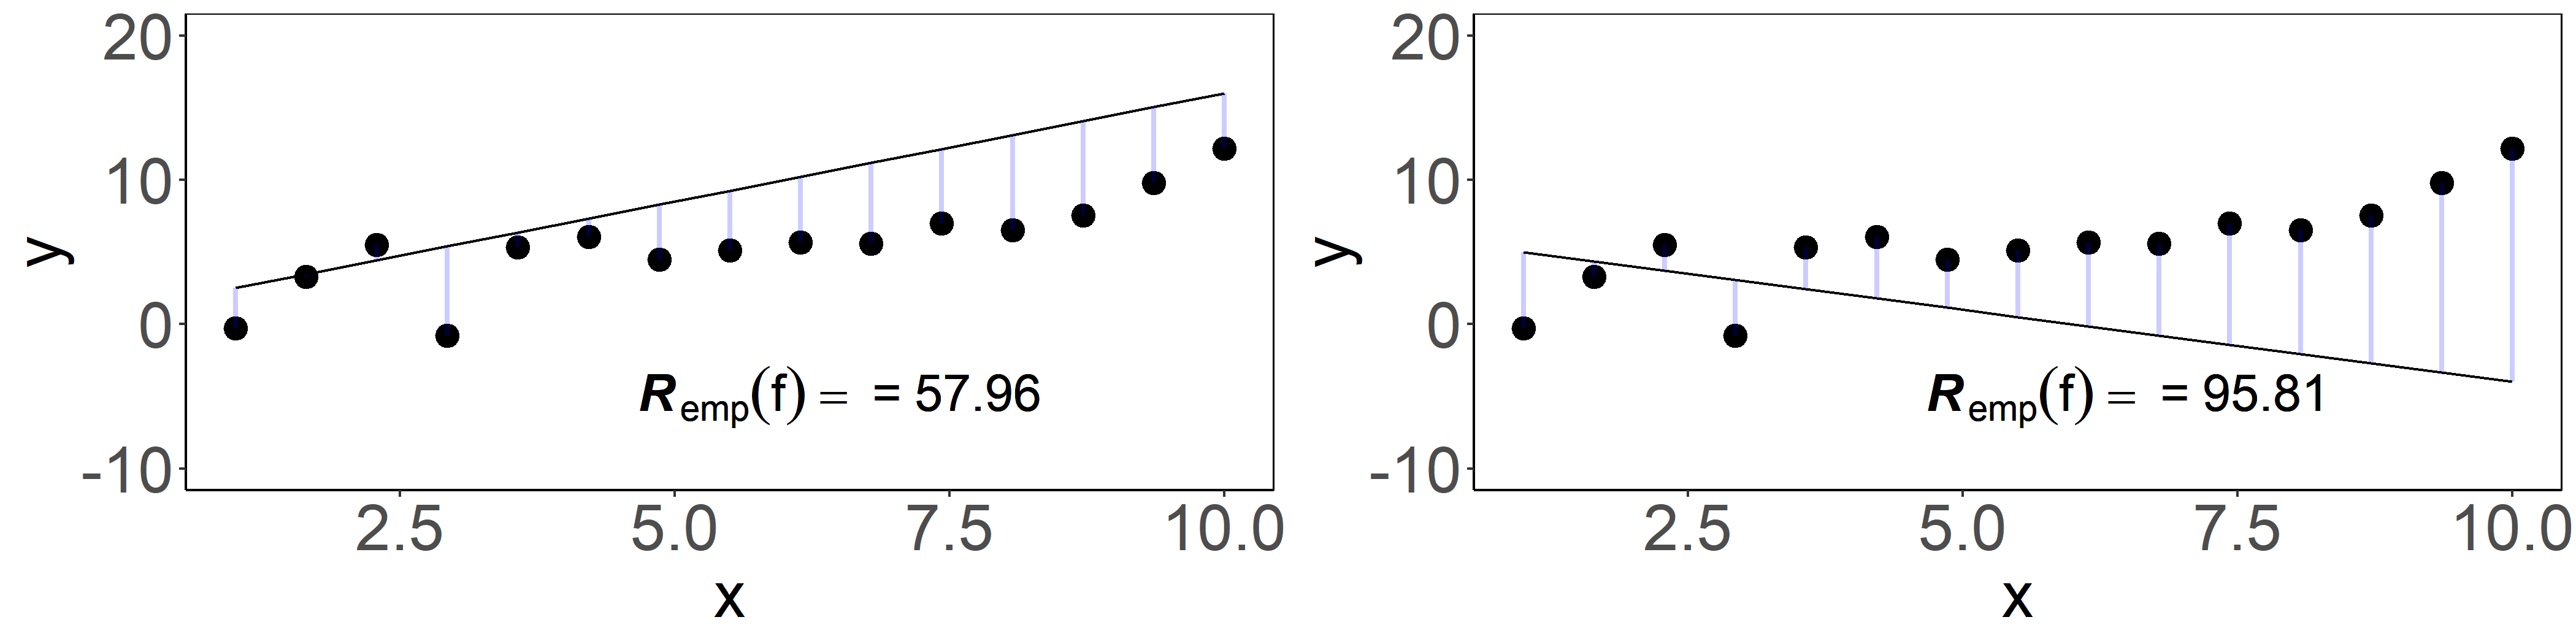
\includegraphics[width=0.9\textwidth]{figure/ml-basic_riskmin-2-risk.png}
\end{figure}
\end{center}

\framebreak 
   
\begin{itemize}
\item The risk can also be defined as an average loss
  $$
    \riskeb(f) = \frac{1}{n}\sumin \Lxyi. 
  $$
  The factor $\frac{1}{n}$ does not make a difference in optimization, so we will consider $\riske(f)$ most of the time.  
\item Since $f$ is usually defined by \textbf{parameters} $\thetab$, this becomes:
$$\risk : \R^d \to \R$$
\begin{eqnarray*}
\risket & = & \sumin \Lxyit \cr
% \thetabh & = & \argmin_{\thetab \in \Theta} \risket
\end{eqnarray*}
 

\end{itemize}
   
   
\end{vbframe}




\begin{vbframe}{Empirical risk minimization}

The best model is the model with the smallest risk. 

\lz

If we have a finite number of models $f$, we could simply tabulate them
and select the best.


% calculated in ml-basic-riskmin-error-surface.R (theta_risk_df)
\begin{center}
\begin{tabular}{ c | c | c || c }
 Model & \(\displaystyle \thetab_{intercept} \) & \(\displaystyle \thetab_{slope} \) & \(\displaystyle \risket \) \\ 
 \hline
\(\displaystyle f_1 \)   & 2 & 3 & 194.62 \\
\(\displaystyle f_2 \)   & 3 & 2 & 127.12 \\  
\(\displaystyle f_3 \)   & 6 & -1 & 95.81 \\
\rowcolor{lightgray}
\(\displaystyle f_4 \)   & 1 & 1.5 & 57.96 \\  
\end{tabular}
\end{center}


\end{vbframe}

\begin{vbframe}{Empirical Risk Minimization}

But usually $\Hspace$ is infinitely large. 

\lz

Instead we can consider the risk surface w.r.t. the parameters $\thetab$.\\
(By this I simply mean the visualization of $\risket$)

\begin{table}
\begin{minipage}{0.4\linewidth}
$$\risket : \R^d \to \R.$$
\scalebox{0.8}{
\begin{tabular}{ c | c | c || c }
 Model & \(\displaystyle \thetab_{intercept} \) & \(\displaystyle \thetab_{slope} \) & \(\displaystyle \risket \) \\ 
 \hline
\(\displaystyle f_1 \)   & 2 & 3 & 194.62 \\
\(\displaystyle f_2 \)   & 3 & 2 & 127.12 \\  
\(\displaystyle f_3 \)   & 6 & -1 & 95.81 \\
\rowcolor{lightgray}
\(\displaystyle f_4 \)   & 1 & 1.5 & 57.96 \\  
\end{tabular}
}
\end{minipage}\hfill
	\begin{minipage}{0.55\linewidth}
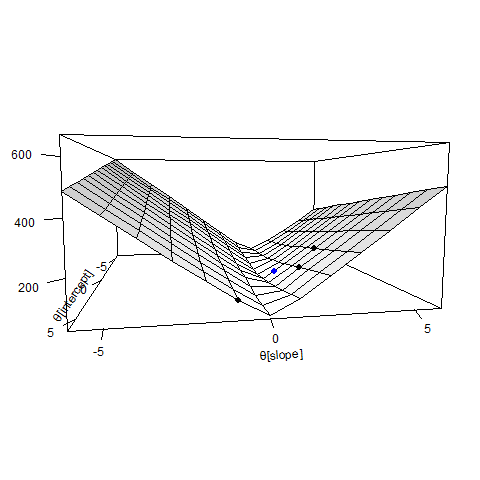
\includegraphics[width=\textwidth]{figure/ml-basic-riskmin-error-surface.png}
\end{minipage}
\end{table}


\framebreak

Minimizing this surface is called \textbf{empirical risk minimization} (ERM).
$$
\thetah = \argmin_{\thetab \in \Theta} \risket.
$$
Usually we do this by numerical optimization.

\begin{table}
\begin{minipage}{0.4\linewidth}
$$\risk : \R^d \to \R.$$
\scalebox{0.8}{
\begin{tabular}{ c | c | c || c }
 Model & \(\displaystyle \thetab_{intercept} \) & \(\displaystyle \thetab_{slope} \) & \(\displaystyle \risket \) \\ 
 \hline
\(\displaystyle f_1 \)   & 2 & 3 & 194.62 \\
\(\displaystyle f_2 \)   & 3 & 2 & 127.12 \\  
\(\displaystyle f_3 \)   & 6 & -1 & 95.81 \\
\(\displaystyle f_4 \)   & 1 & 1.5 & 57.96 \\ 
\rowcolor{lightgray}
\(\displaystyle f_5 \)   & 1.25 & 0.90 & 23.40 \\ 
\end{tabular}
}
\end{minipage}\hfill
	\begin{minipage}{0.55\linewidth}
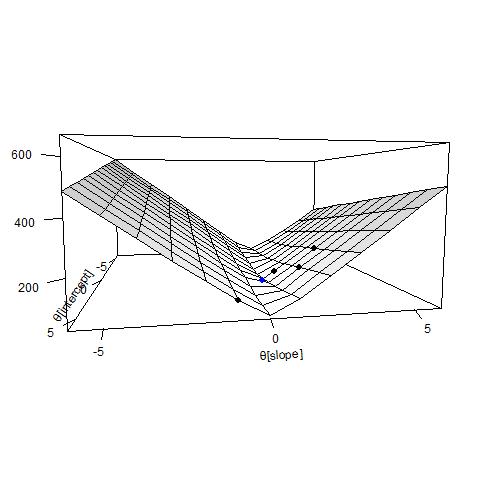
\includegraphics[trim=0 100 0 100,clip,width=\textwidth]{figure/ml-basic-riskmin-error-surface-best.png}
\end{minipage}
\end{table}

In a certain sense, we have now reduced the problem of learning to 
\textbf{numerical parameter optimization}.

\end{vbframe}


% \begin{vbframe}{Further remarks}
% \begin{itemize}
% \item For regression tasks, the loss often only depends on the residual $\Lxy = L(y - \fx) = L(\eps)$.
% \item The choice of loss implies which kinds of errors are important or not -- requires \emph{domain knowledge}!
% \item For learners that correspond to probabilistic models, the loss determines / is equivalent to distributional assumptions.
% \item Since learning can be re-phrased as minimizing the loss, the choice of loss strongly affects the computational difficulty of learning:
% \begin{itemize}
%     \item How smooth is $\risket$ in $\thetab$?
%     \item Is $\risket$ differentiable so that we can use gradient-based methods?
%     \item Does $\risket$ have multiple local minima or saddlepoints over $\Theta$?\\
% \end{itemize}

% \end{itemize}
% \end{vbframe}



\endlecture

\end{document}
